Tackling the objectives laid out in \cref{sec:navig-virt-subsyst-design} requires an organized and well thought-out plan of work because there are a lot of smaller systems at play that need to work cohesively and synchronously. 




%///////////////////////// # Separation into packages //////////////////////////

The best way to achieve a good plan is by first separating the problem into packages, and in each package have subpackages, each with a collection of modules dedicated to serve a collective purpose in the data treatment and organization chain. 

The system is divided into such packages as follows:

\begin{figure}[H]
	\centering
	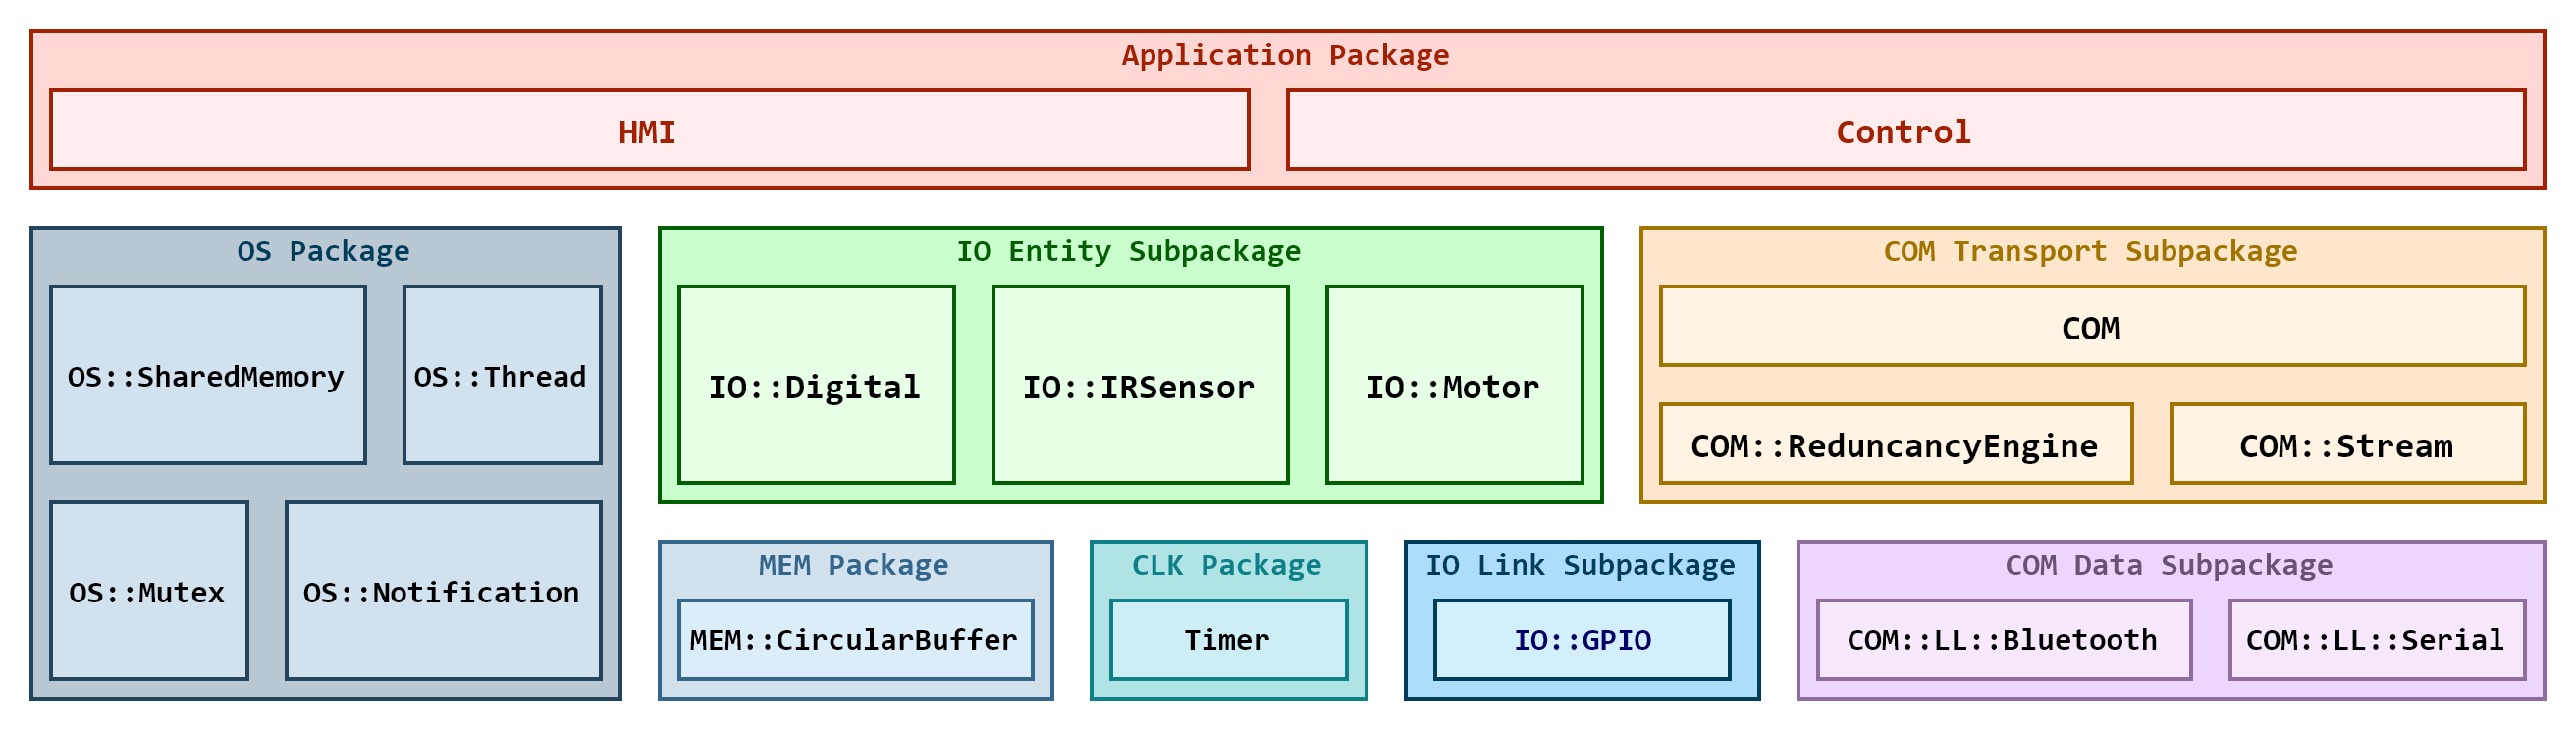
\includegraphics[width=1.0\textwidth]{./img/full-stack-overview.png}
	\caption {Full Stack Overview}
	\label{fig:full-stack-overview}
	\end{figure}
	


%////////////////////////// # Separation into layers ///////////////////////////

Each subpackage also belongs to a certain layer of software, characterized not by the resources it is associated to but by how close the modules within it are to the hardware. Futhermore, the packages should be distributed between layers in such a way that one seldomly need to use another that doesn't belong to the same layer or the layer directly below. 

These layers are, from the bottom to the top:
\begin{itemize}
	\item The High-level Hardware Abstraction Layer, which consists of the \textbf{OS} (partly), \textbf{MEM}, \textbf{CLK}, \textbf{IO Link} and \textbf{COM Data} packages/subpackages. Modules within this layer are responsible for the lower-level interaction with the system's resources so they are made to be thread-safe. Their implementation is platform-dependent and their interface is platform-agnostic. The main goal for this layer of software is to standardize the hardware, making for clean, maintainable and easily portable code. 
	\item The High-level Software Abstraction Layer, consisting of the \textbf{OS} (partly), \textbf{IO Entity} and \textbf{COM Transport} packages. The modules within these packages should serve as an interface with the lower level layer, creating a more intuitive interaction process and mechanisms for processing information asynchronously. This way, when other modules make use of those interfaces, the information is already parsed and ready to be retrieved.\\
	Modules in the layers above ara also highly dependent on both abstraction layers to carry out their tasks in time so the ones in this layer should provide robust mechanisms for exception-handling and timing. 
	\item The Main Application Layer, comprised only of the \textbf{APP} package, where the core functionality lies. As stated earlier, modules in this layer are protected from having to access to most lower-level layers but can use those modules and must use when no other abstraction is provided.
\end{itemize}




%//////////////////////////////// # IO Package /////////////////////////////////
\subsubsection{IO: Input/Output Package}

The \textbf{IO} package is comprised of the \textbf{IO Entity} and \textbf{IO Link} subpackages. The modules within these subpackages are the parts of the hardware abstraction layers responsible for standardizing the General Purpose Input/Output resources of the machine.

\begin{figure}[H]
	\centering
	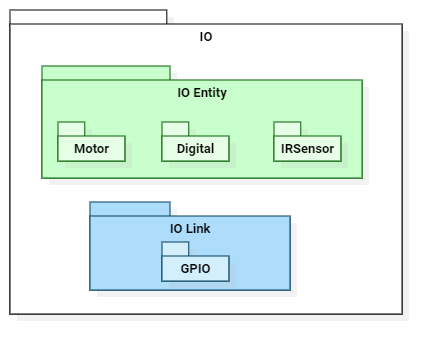
\includegraphics[width=0.5\textwidth]{./img/package-diagram-io.png}
	\caption {IO Package Diagram}
	\label{fig:navig-package-diagram-io}
	\end{figure}


The \textbf{IO Link} subpackage is the interface provides the most generic yet complete package for interacting with the machine. It provides such functionality as automatic resource assignment, automatic buffering or timed output/input.

The \textbf{IO Entity} subpackage serves for specialization of functionality present in \textbf{IO Link} to serve a certain purpose attached to a physical meaning. This means it also provides methods for automatic calculation of real-world values based on the measurements taken or otherwise.

\begin{figure}[H]
	\centering
	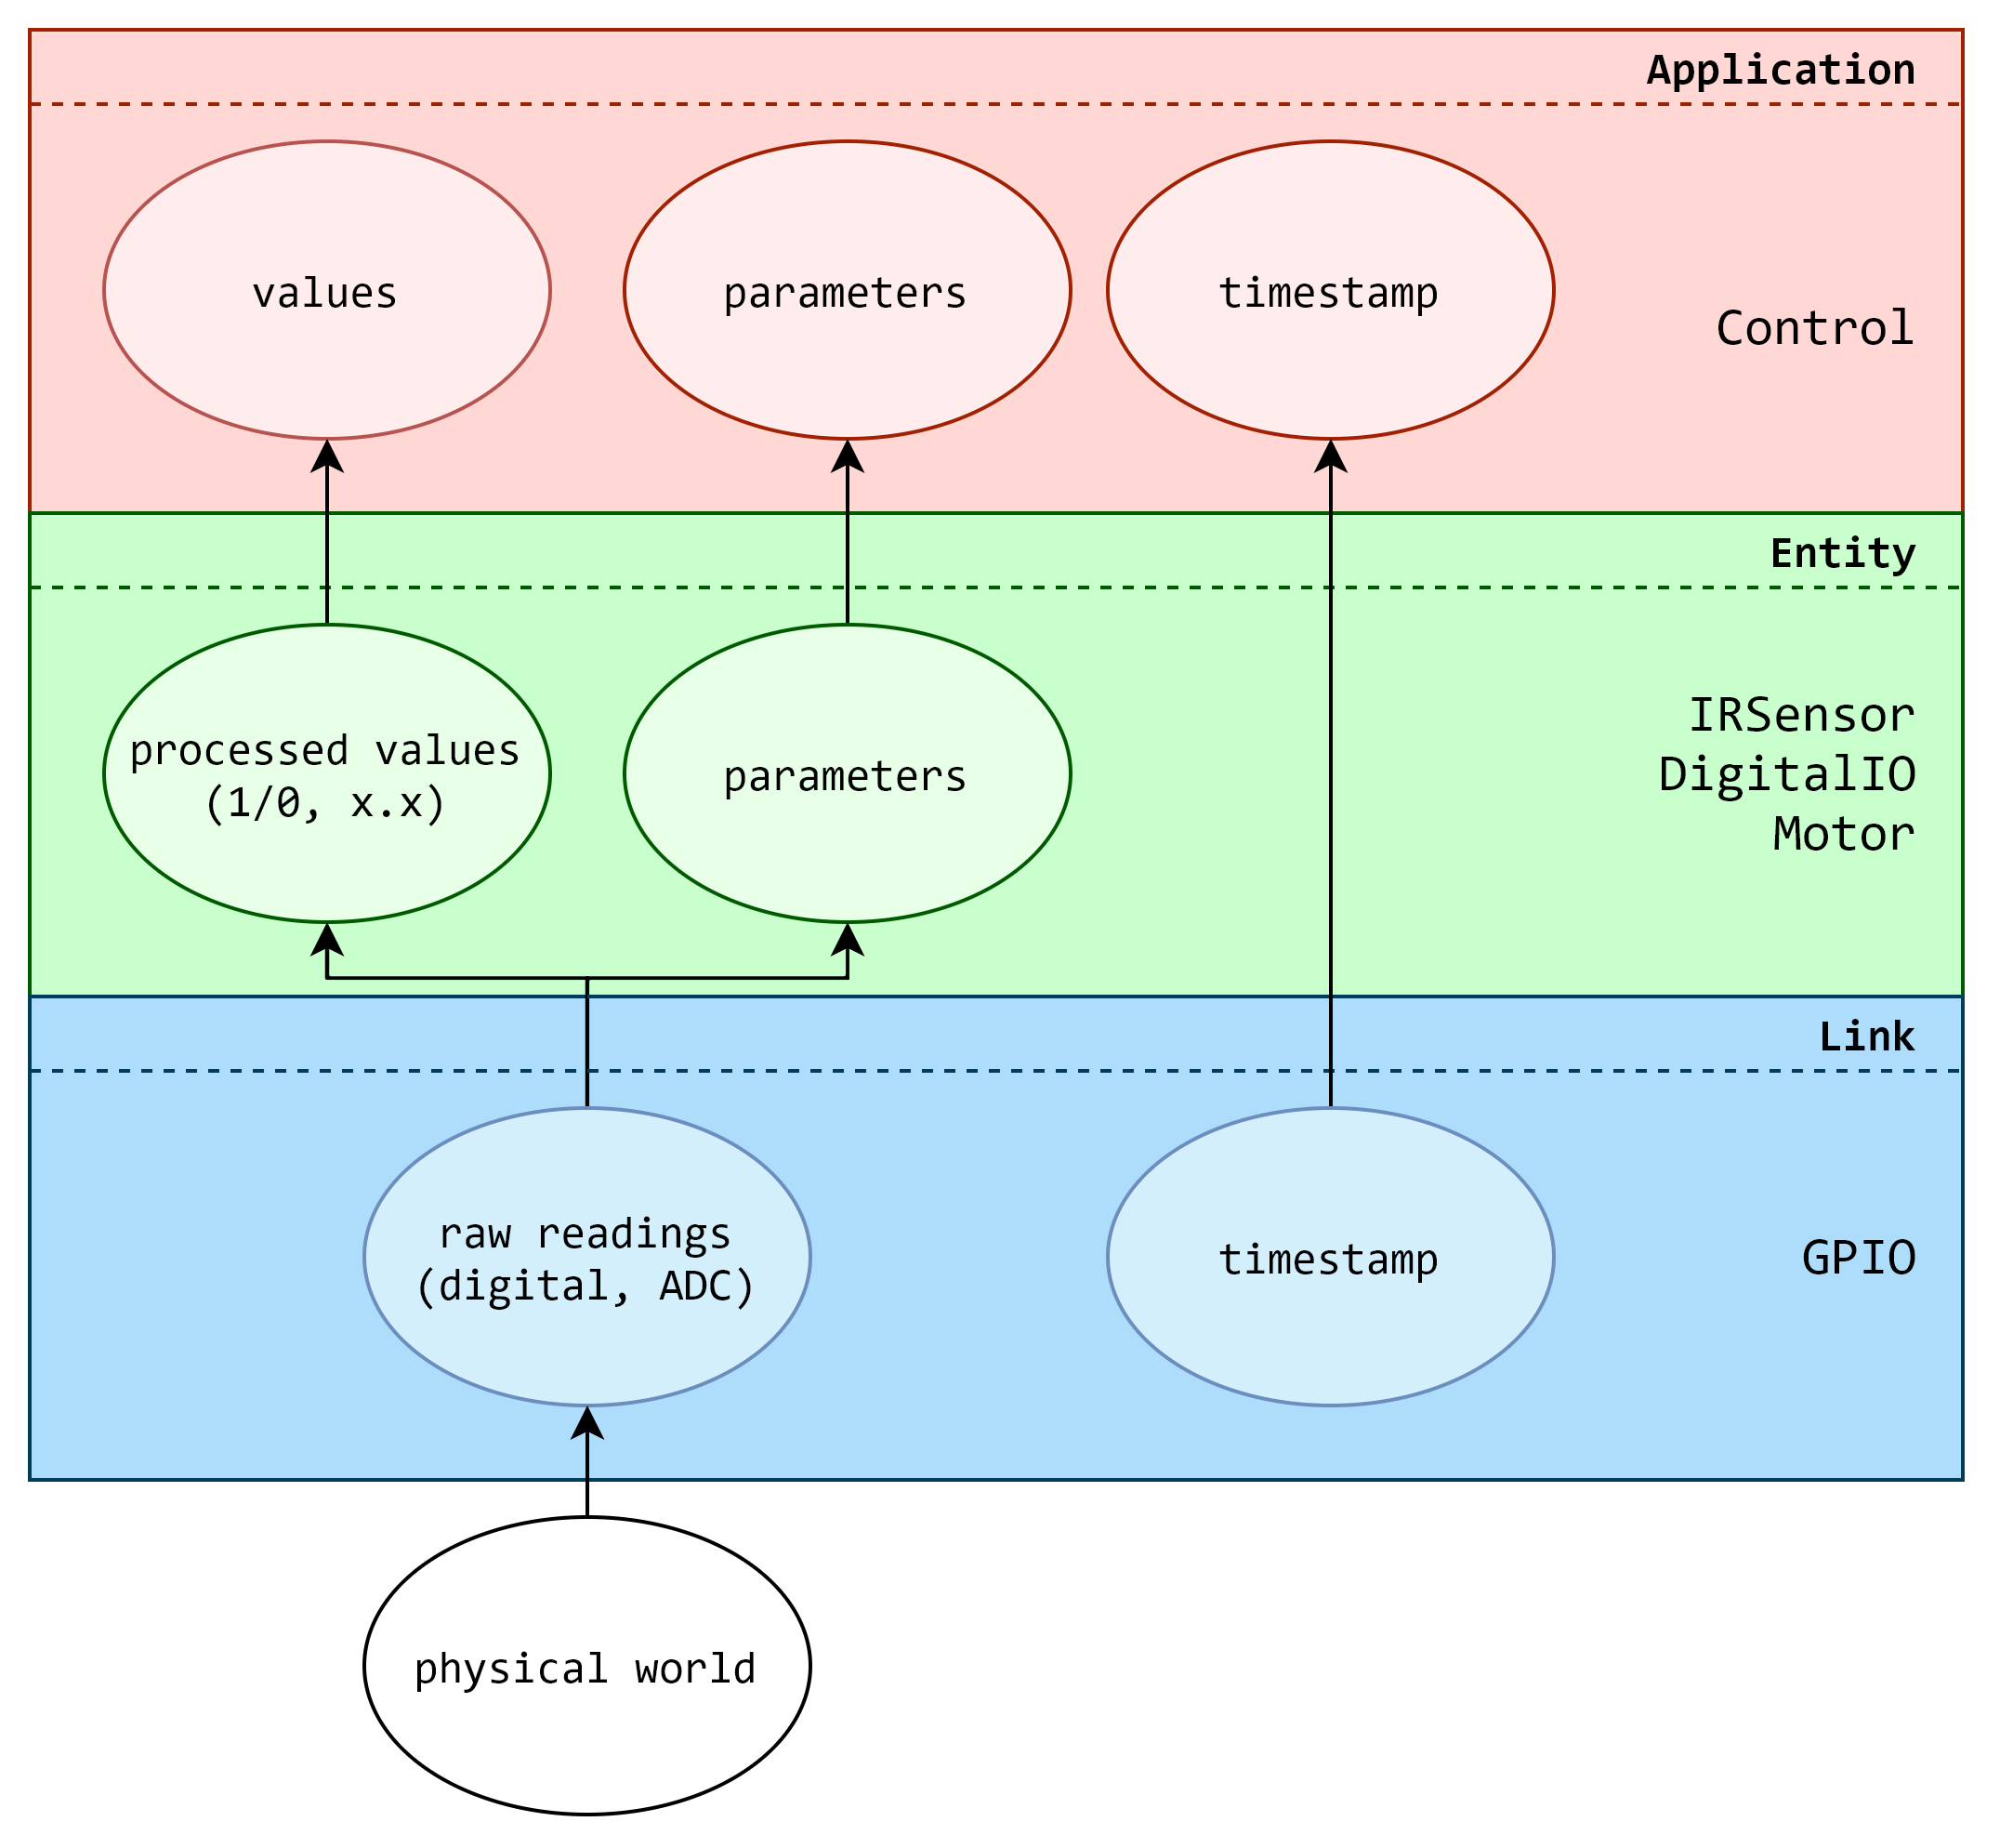
\includegraphics[width=0.5\textwidth]{./img/module-stack-io.png}
	\caption {IO subpackage interaction and information propagation diagram}
	\label{fig:navig-module-stack-io}
	\end{figure}


%//////////////////////////////// # COM Package ////////////////////////////////
\subsubsection{COM: Communications Package}

The COM package is the sum of the COM Data and COM Transport subpackages. These  modules are responsible for standardizing the access to the inter-device communication resources of each machine. 

\begin{figure}[H]
	\centering
	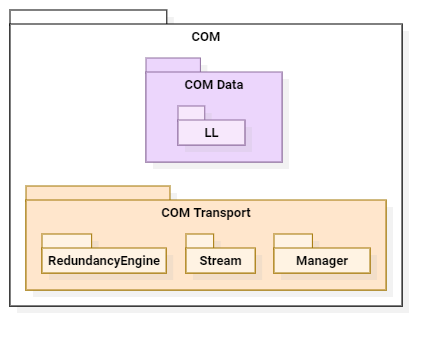
\includegraphics[width=0.5\textwidth]{./img/package-diagram-com.png}
	\caption {COM Package Diagram}
	\label{fig:navig-package-diagram-com}
	\end{figure}


The \textbf{COM Data} subpackage is aimed at providing a platform-agnostic interface for communicating over a serial or Bluetooth connection, while also providing specific functionality for different protocols/roles.
The \textbf{COM Transport} subpackage provides tools for managing multiple simultaneous, redundant, multiprotocol and multi-stream connections as well as automatically parsing of data for usage in time-constrained scenarios.

\begin{figure}[H]
	\centering
	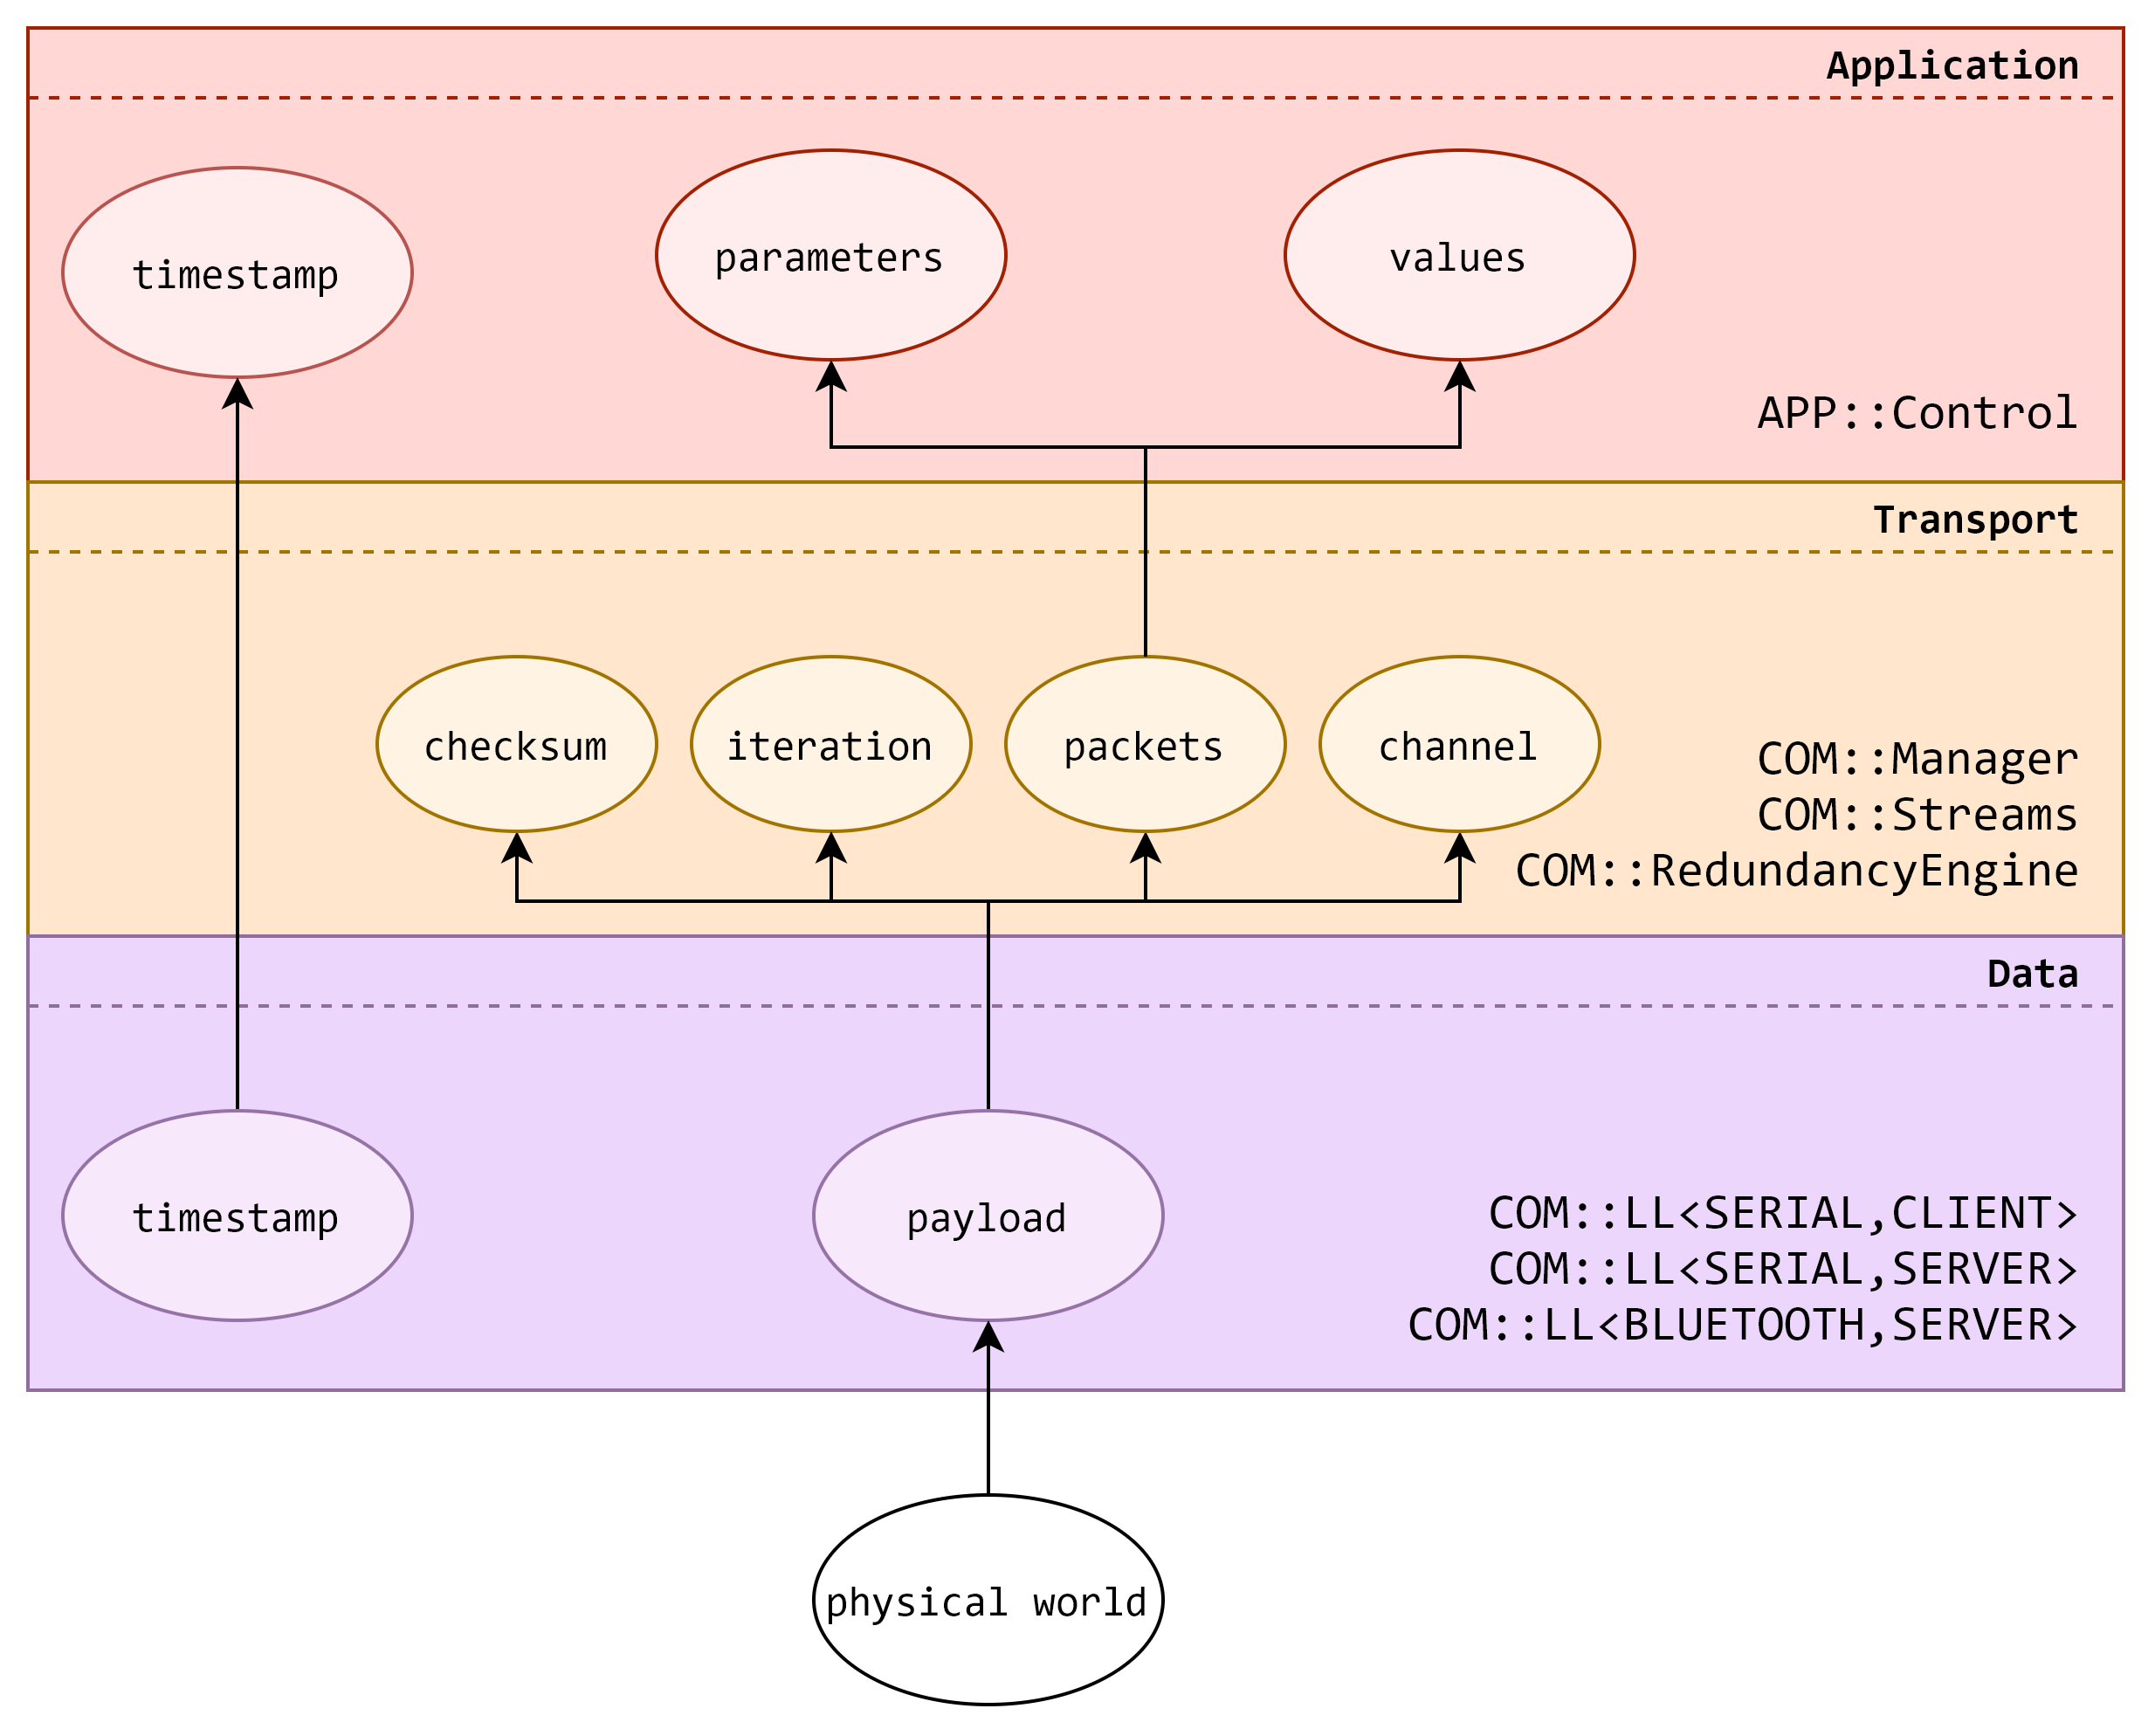
\includegraphics[width=0.5\textwidth]{./img/module-stack-com.png}
	\caption {COM subpackage interaction and information propagation diagram}
	\label{fig:navig-module-stack-com}
	\end{figure}
	

%//////////////////////////////// # OS Package /////////////////////////////////
\subsubsection{OS: Scheduler Package}

The modules in the OS package mainly serve the purposes of thread creation and management management, inter-thread synchronization and thread-safe access to memory.

\begin{figure}[H]
	\centering
	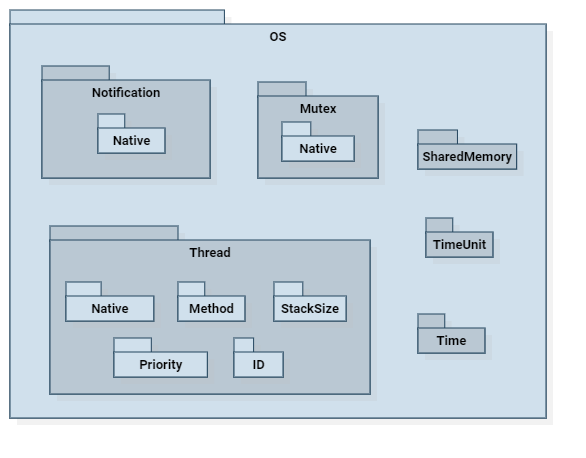
\includegraphics[width=0.5\textwidth]{./img/package-diagram-os.png}
	\caption {OS Package Diagram}
	\label{fig:navig-package-diagram-os}
	\end{figure}



\subsubsection{MEM: Memory Structures Package}
\subsubsection{CLK: Timing Package}
\subsubsection{APP: Main Application Package}

